%-----------------------------------------------------------------------------80
% CONTENT
%-----------------------------------------------------------------------------80

\subsection{Compilación}

\begin{frame}[fragile]{Compilación}
\textbf{Compilador}
  \begin{itemize}[<+(1)->]
  \item Programa  escrito en un lenguaje de programación, que a su vez, traduce y genera otro programa
en otro lenguaje de programación (código máquina), ambos equivalentes.
  \item En principio, al usar un compilador, se busca traducir y simplificar un lenguaje de mayor complejidad a uno mucho más cotidiano y manejable en términos informáticos.
 \end{itemize}
\end{frame}


\begin{frame}[fragile]{Compilación} 
  \begin{figure}
    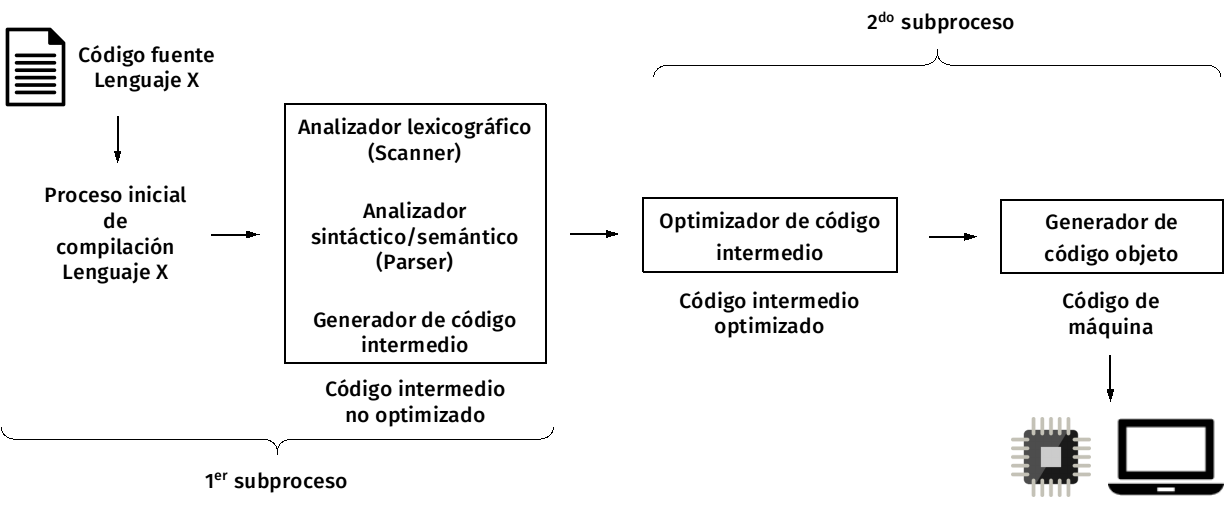
\includegraphics[width=1\textwidth]{./resources/compilation_op.png}
    \caption{Diagrama de bloques del proceso de compilación}
   \end{figure}
\end{frame}


\begin{frame}[fragile]{Compilación}
\textbf{Proceso de compilación}
  \begin{itemize}[<+(1)->]
  \item  
     
  \item []El compilador de fortran posee la siguiente sintaxis:
  \item [] 
     \begin{mintedbash} 
      fcomp [opciones] file1 [file2] [...] [fileN]
     \end{mintedbash}
  \item [-] fcomp $~$ denota el comando para llamar al compilador. (gfortran, ifort, ...)
  \item [-] opciones $~$ opciones que permite el compilador. (-o, -f, -c, ...)
  \item [-] file $~$ denota el archivo con su respectiva extensión (.f90, .f95, .o, ...)    
  \end{itemize}

\end{frame}